\documentclass{chi-ext}
% Please be sure that you have the dependencies (i.e., additional LaTeX packages) to compile this example.
% See http://personales.upv.es/luileito/chiext/

%% EXAMPLE BEGIN -- HOW TO OVERRIDE THE DEFAULT COPYRIGHT STRIP -- (July 22, 2013 - Paul Baumann)
% \copyrightinfo{Permission to make digital or hard copies of all or part of this work for personal or classroom use is granted without fee provided that copies are not made or distributed for profit or commercial advantage and that copies bear this notice and the full citation on the first page. Copyrights for components of this work owned by others than ACM must be honored. Abstracting with credit is permitted. To copy otherwise, or republish, to post on servers or to redistribute to lists, requires prior specific permission and/or a fee. Request permissions from permissions@acm.org. \\
% {\emph{CHI'14}}, April 26--May 1, 2014, Toronto, Canada. \\
% Copyright \copyright~2014 ACM ISBN/14/04...\$15.00. \\
% DOI string from ACM form confirmation}
%% EXAMPLE END -- HOW TO OVERRIDE THE DEFAULT COPYRIGHT STRIP -- (July 22, 2013 - Paul Baumann)

\title{Drunken Ed - A Balance Game For Public Large Screen Displays}

\newcommand{\tuaddr}{
\affaddr{Technische Universit\"at Berlin}\\
\affaddr{Stra\ss e des 17. Juni 135}\\
\affaddr{Berlin, 10623 Germany}\\
}

\numberofauthors{5}
% Notice how author names are alternately typesetted to appear ordered in 2-column format;
% i.e., the first 4 autors on the first column and the other 4 auhors on the second column.
% Actually, it's up to you to strictly adhere to this author notation.
\author{
	\alignauthor{
  	\textbf{Jonas Willaredt}\\
  	\tuaddr
  	\email{jonas.willaredt@campus.tu-berlin.de}
  }\alignauthor{
  	\textbf{Andreas Fender}\\
  	\tuaddr
  	\email{andreas.fender@campus.tu-berlin.de}
  }
  \vfil
  \alignauthor{
  	\textbf{Tiare Feuchtner}\\
  	\tuaddr
  	\email{tiare.feuchtner@campus.tu-berlin.de}
  }\alignauthor{
  	\textbf{Marcel Karsten}\\
  	\tuaddr
  	\email{marcel.karsten@campus.tu-berlin.de}
  }
  \vfil
	\alignauthor{
  	\textbf{Alexander Biskupski}\\
  	\tuaddr
  	\email{alexander.biskupski@campus.tu-berlin.de}
  }
}

% Paper metadata (use plain text, for PDF inclusion and later re-using, if desired)
\def\plaintitle{Drunken Ed - A Balance Game For Public Large Screen Displays}
\def\plainauthor{Alexander Biskupski, Andreas Fender, Tiare Feuchtner, Marcel Karsten, Jonas Willaredt}
\def\plainkeywords{Public displays, large screen display, casual game, balance game, natural user interface, kinect, gesture control}
%\def\plaingeneralterms{Documentation, Standardization}

\hypersetup{
  % Your metadata go here
  pdftitle={\plaintitle},
  pdfauthor={\plainauthor},  
  pdfkeywords={\plainkeywords},
 % pdfsubject={\plaingeneralterms},
  % Quick access to color overriding:
  %citecolor=black,
  %linkcolor=black,
  %menucolor=black,
  %urlcolor=black,
}

\usepackage{graphicx}   % for EPS use the graphics package instead
\usepackage{balance}    % useful for balancing the last columns
\usepackage{bibspacing} % save vertical space in references

\usepackage{graphicx}

\newcommand{\drunkened}{\textit{Drunken Ed}}
\newcommand{\ed}{Ed}
\newcommand{\eds}{Ed's}
\newcommand{\lbreak}{\\[0.7cm]}

\newcommand{\image}[2]{
\begin{center}
\includegraphics[scale = #1]{pictures/#2}
\end{center}
}
\newcounter{imgcounter}
\newcommand{\figimage}[4]{
\begin{figure}[h] 
\image{#1}{#2}
\caption{\textit{#3}\\#4}
\label{#2}
\end{figure}
}
\newcommand{\capimage}[3]{
\begin{center}
\includegraphics[scale = #1]{#2}\\
\begin{small}#3\end{small}
\end{center}
}

\begin{document}

\maketitle

\begin{abstract}
\drunkened\ is a 2D balance game that was specifically designed for public displays. We show that this casual game is well suited for public context and that camera based body tracking offers convenient interaction techniques for large screen displays. This single player game has a very direct control mapping, which uses the orientation of the player's torso in relation to the ground to help Ed keep balance in a wobbling world. Ed's body pose reflects that of the player, creating a very direct form of control. In addition we apply the simple gesture of raising a hand to the mouth to drink, to trigger a selection in the menu. In our evaluation this form of mapping has proven to be very intuitive and the short play sessions agree with the requirements of a casual game in public environment. Furthermore the game setting is widely accepted, despite its drunken protagonist.
%Do not change the page size or page settings.
\end{abstract}

\keywords{\plainkeywords}

\category{H.5.m}{Information interfaces and presentation (e.g., HCI)}{Miscellaneous}. 


% =============================================================================
\section{Introduction}
% =============================================================================
The balance game \drunkened\ was developed with the goal of creating an application for public large screen displays, which could provide some sort of entertainment. Games are intrinsically motivating \cite{salen2004rules} \cite{malone1981motivation}, thus it is not required that the application fulfills any further useful purpose. By designing the game for a large screen display with vision based body tracking for the controls, \drunkened\ can be easily installed in a public area, such as a waiting room, where it serves to entertain, relieve boredom and shorten the wait.
The gameplay of \drunkened\ can be briefly described as a single player game, with the mission to guide Ed home safely. Ed has had a couple of drinks too many, and dangerously staggers along the sidewalk. The player must lean left and right to help Ed keep balance and avoid obstacles, as depicted in [\ref{??}].
To ensure suitability for public context, we strove to fulfill the criteria of acceptability, accessibility, simplicity and flexibility as proposed by \cite{kultima2009casual}. \textit{Acceptability} was a strongly discussed aspect, since our protagonist Ed indulges in the pleasure of consuming alcohol, which causes him to stagger along the streets drunkenly. However we have found that this situation is widely accepted and considered fun, specially among young people. The questioned subjects responded that they could easily relate to this situation and described the experience of steering Ed as entertaining. Furthermore our game does not encourage people to drink, but points out the problematic consequences of drinking too much. \textit{Accessibilty} is guaranteed by our physical setup with a large screen and visual tracking. The game can be played by anybody who approaches it, independent of sex size, or age. However the tracking capability of the Kinect sets a couple of limitations, such as inability to cope with occlusion and bad lighting situations. \textit{Simplicity} is given by keeping the components of the game minimal and providing the user with a single main control mechanic - bending the upper body left and right in order to help Ed keep balance. Finally \textit{flexibility} is ensured by forgiving mistakes and gracefully recovering from situations such as when the player suddenly leaves the traking area.
The starting point of the game, is the minimalistic level selection menu displaying Ed in a pub shown in figure \ref{??}. Here the player may experiment with the controls and make Ed stagger left and right by leaning. On the counter there are three different types of alcohol: Beer, Wine and Vodka. The player can make Ed drink one of these by positioning Ed accordingly and performing a drinking gesture. This component of choice entails a further motivation factor according to Malone \cite{malone1981motivation}. Animations and hints inform the player about his options. Upon drinking, the game starts and Ed begins his unsteady way home. The difficulty of the selected level depends on the type of drink consumed - stronger alcohol makes it more difficult for Ed to keep balance. The difficulty further increases with time. A counter informs the player about his progress. Upon losing balance and falling down, a highscore list is shown. If the player has managed a top score, he can have his picture taken to be displayed on the list. Ed never actually reaches his home, thus this is purely an endurance game with the goal of getting as far as possible. We hereby allow players who approach in groups to compete with their friends for the best scores. \cite{ohara2008understanding}


%\drunkened\ is a 2D balance game specifically designed for public displays. The player stands in front of a large display and is tracked by a Kinect. By bending his or her own upper body, the player steers a drunkyard called \textit{\ed}. The goal of the game is to walk as far as possible without falling down. While the time passes, the difficulty increases contineously. So the player has to keep the balance to not fall down, but at the same time, he or she has to hurry because it is getting harder and harder to increase the walked distance.\\
One key element of the visuals is the rotating camera: many balance games keep the world static while letting the player balance an object. In this game, the opposite is the case: it is the world around the figure, which needs to be balanced with respect to the upper body. 


%third person, but subjective

% =============================================================================
\section{Game Play and Mechanics}
% =============================================================================
As long as no player stands in front of the screen, a bar is shown together with three blackboards containing the highscores. A hint invites the player to step onto the mark, which is located in front of the screen. When a player is detected, the main protagonist \ed appears. The player can now get used to the controls, without having to worry about balancing yet. At the same time, the player chooses the difficulty, encoded as three different alcoholic drinks: beer, wine and wodka. By bending him or herself, the player can move \ed\ to the respective drink. The user confirms his or her choice by doing a drink gesture.\lbreak

Afterwards, the main game starts. The player must make \ed\ walk as far as possible to the right. \ed\ does not walk in a controlled manner, but always follows his center of mass. This resembles a typical accentuated movement of a drunken person. The player bends his or her upper body to control \eds\ upper body, which in turn shifts his center of mass. \ed\ gets faster, the more he bends. The core mechanic is the rotating world: The upper body of \ed\ has the same orientation as of the player with respect to the screen, but not with respect to the rotating world around \ed. Therefore, the player must compensate the world's rotation to not tumble, which happens as soon as the angle between the upper body and the floor gets too narrow. Alternatively, \ed\ tumbles by getting to fast.\\
The higher the difficulty, the faster and uncontrollable the world rotates, which makes it hard to hold the balance and move to the right at the same time.\lbreak

\ed\ will eventually fall down. The game over overlay appears and the distance \ed\ walked until falling down is presented to the player. The distance is the score. If the player got a top three score, he or she can take a picture of him or herself to appear in the highscore list of the bar. The player does so by doing the drink gesture, in order that the picture captures him or her in a drinking posture. If the player does not want to take a picture, he or she has to wait for some seconds without doing anything or to leave the play area. Afterwards, the game restarts and the player gets back to the difficulty selection.\lbreak

During gameplay, the arms of \ed\ play an important role: In the difficulty selection, the arms are controllable by the players arms. However, in the main game, resembling typical cartoony postures of drunkyards, the arms are saggy, pointing straight towards the floor. Firstly, this emphasizes the loss of physical control, because the players arm movements are ignored now. Furthermore, they contribute to the players orientation, because \eds\ arms being aligned with the upper body mean a neutral posture without movement. When they are not aligned, the angle helps estimating the movement. In addition, the arms have an important feedback role: if \ed\ is getting too fast, they start to flail. If \ed\ is about to overbend, they start to swing. Players quickly understood those actions as alarming indicators.

% =============================================================================
\section{Design Principles}
% =============================================================================
Since \drunkened\ is a public display game, it has to have several properties:
\begin{itemize}\compresslist
\item It must be very easy to understand and to play. Therefore, the game is reduced to one main input (the upper body) and one simple goal (walking to the right).
\item One game session must be quite short. The game and also public display games in general are targeting people, which are actually not planning to play. Therefore, they might not want to spent to much time with a game, that they started spontaneously. Furthermore, \drunkened\ is a single player game, so players have to take turns, which is easier with short game sessions.
\marginpar{
\begin{figure}
  \centering
  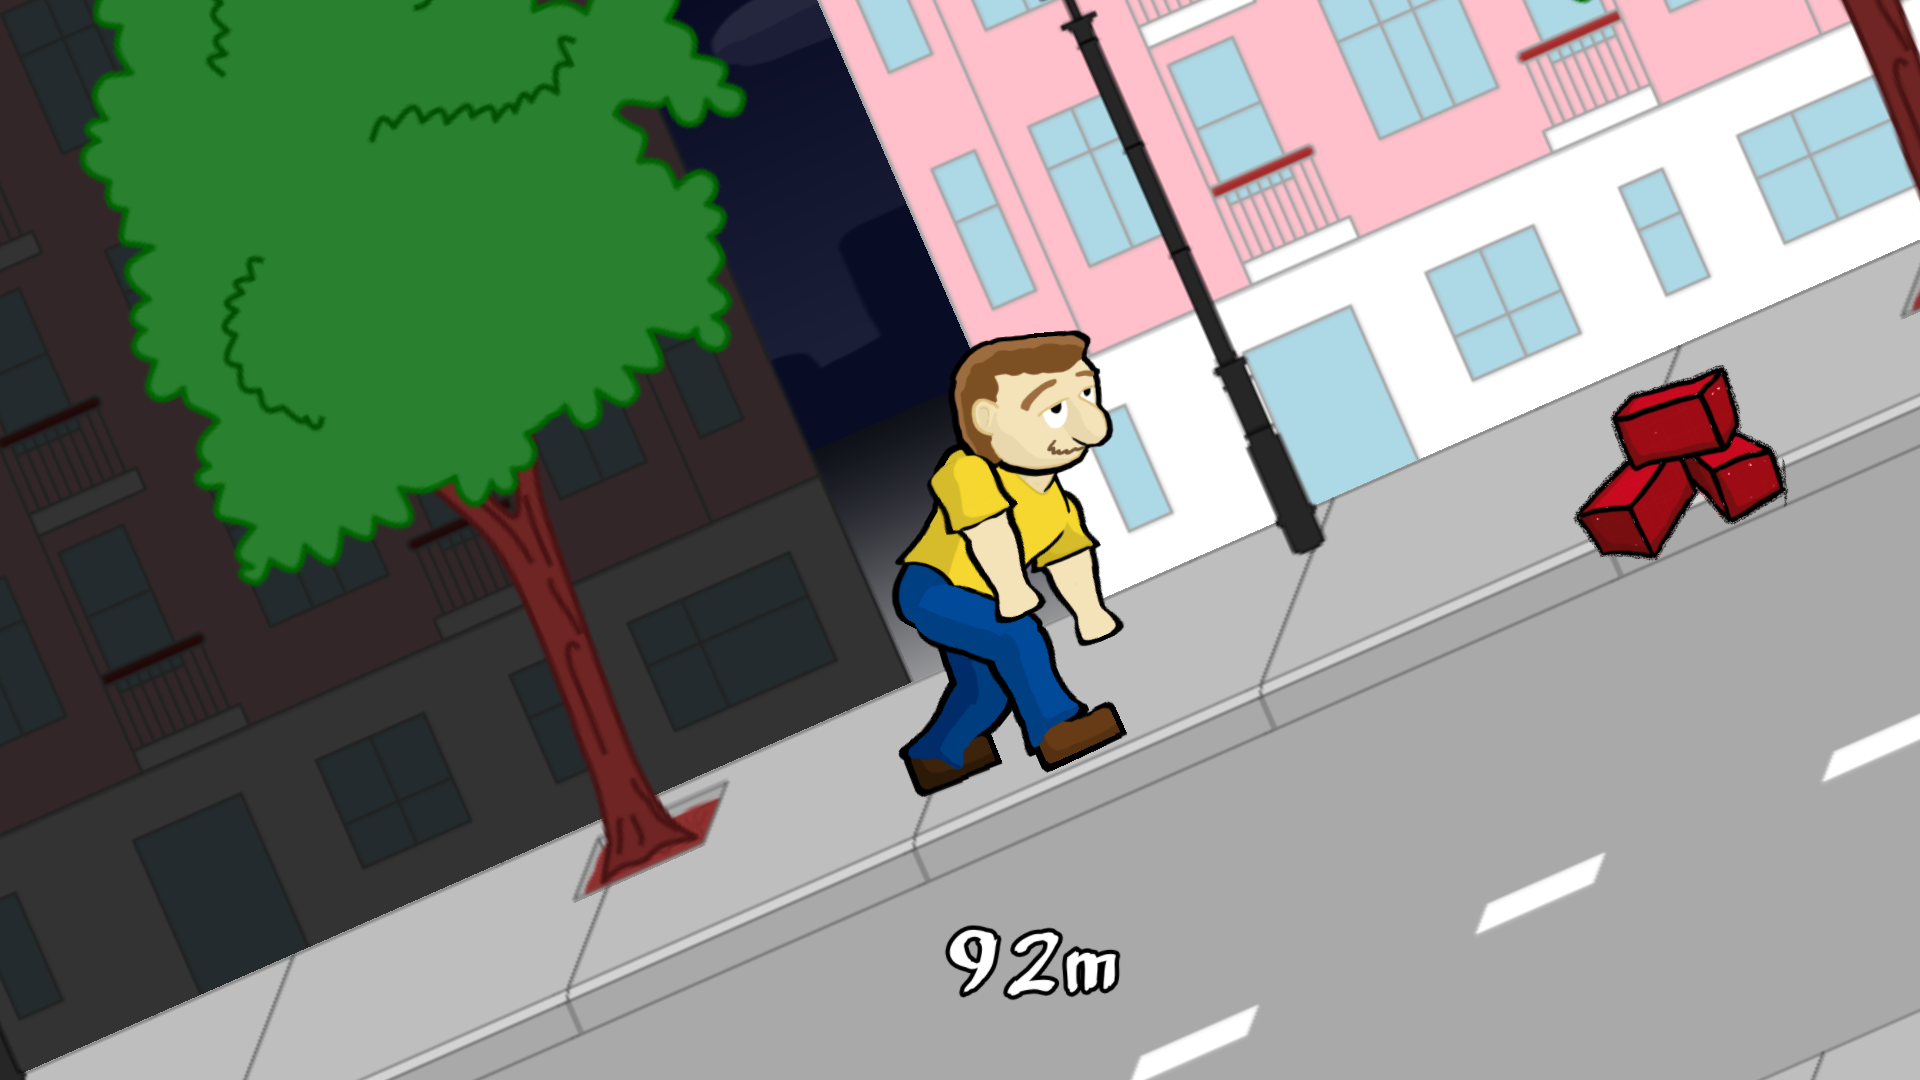
\includegraphics[width=\linewidth]{pictures/screenshot1.png}
  \caption{Insert a caption below each figure.}
  \label{fig:screenshot1}
\end{figure}
\begin{figure}
  \centering
  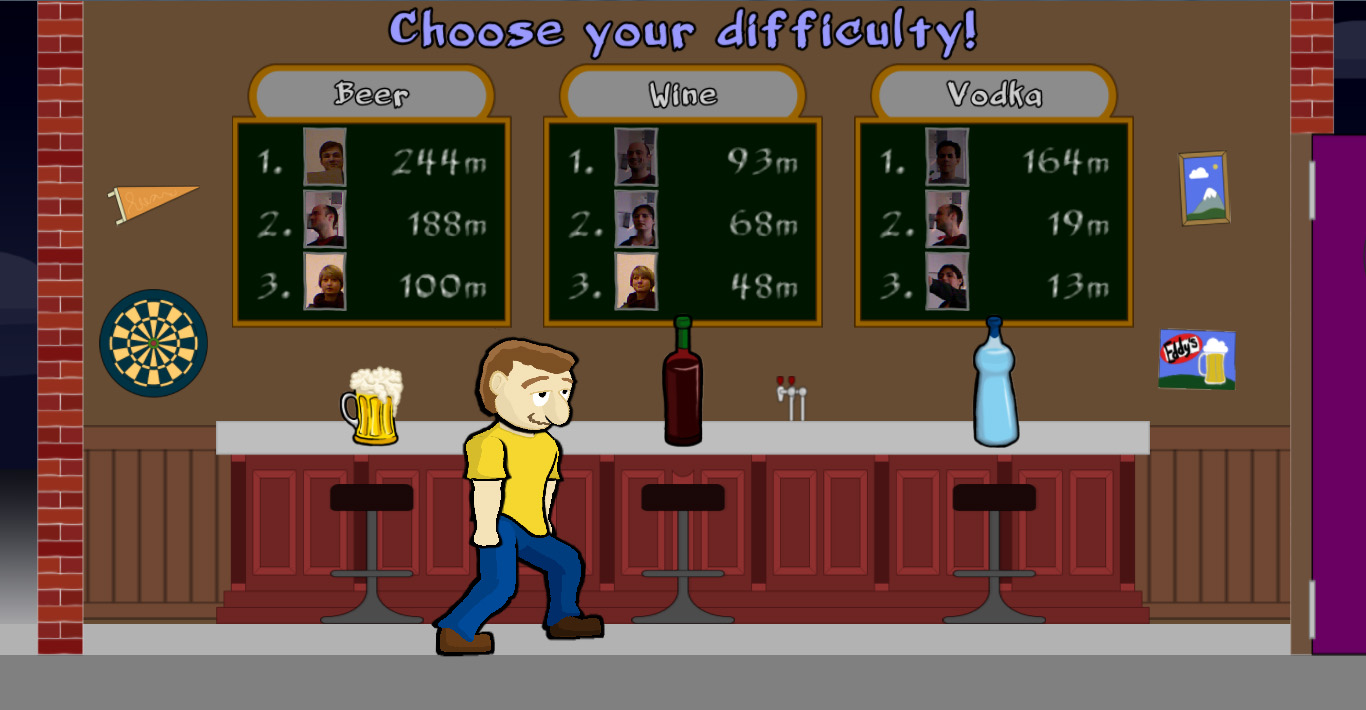
\includegraphics[width=\linewidth]{pictures/screenshot2.jpg}
  \caption{Insert a caption below each figure.}
  \label{fig:screenshot2}
\end{figure}
\begin{figure}
  \centering
  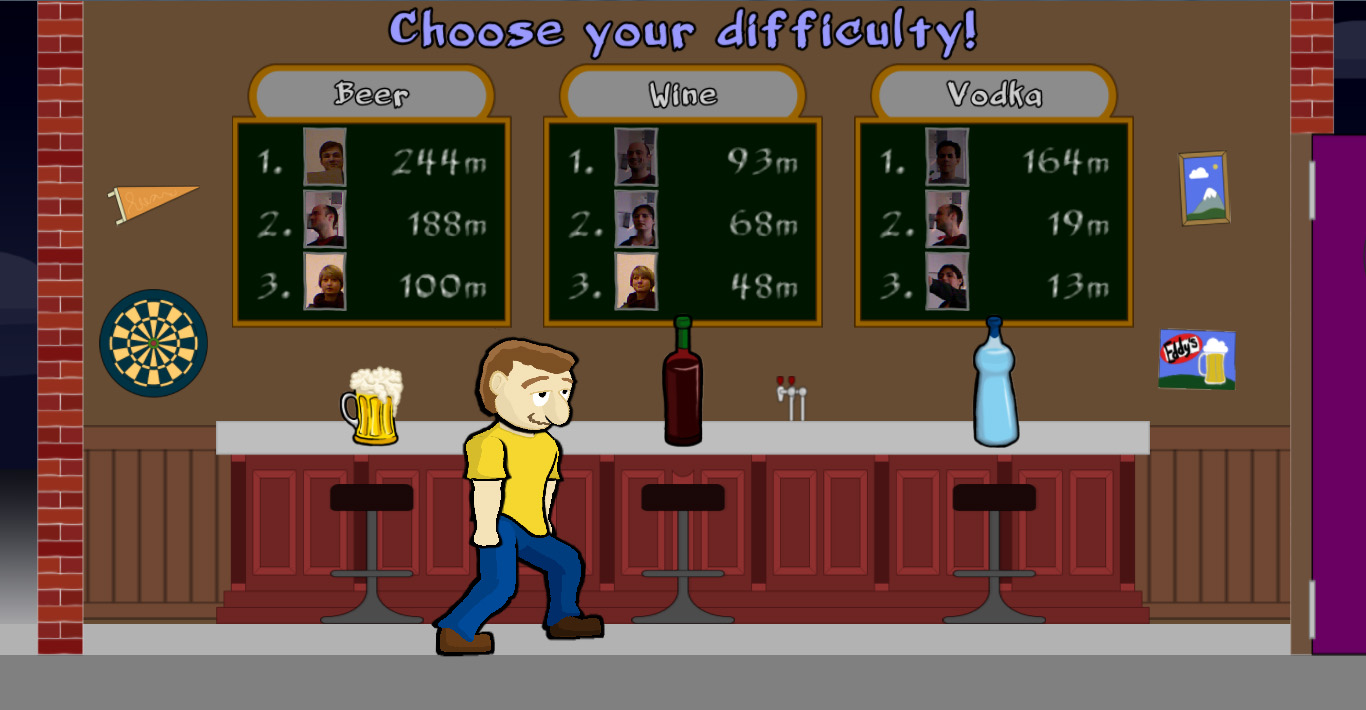
\includegraphics[width=\linewidth]{pictures/screenshot2.jpg}
  \caption{Insert a caption below each figure.}
  \label{fig:screenshot3}
\end{figure}
\begin{figure}
  \centering
  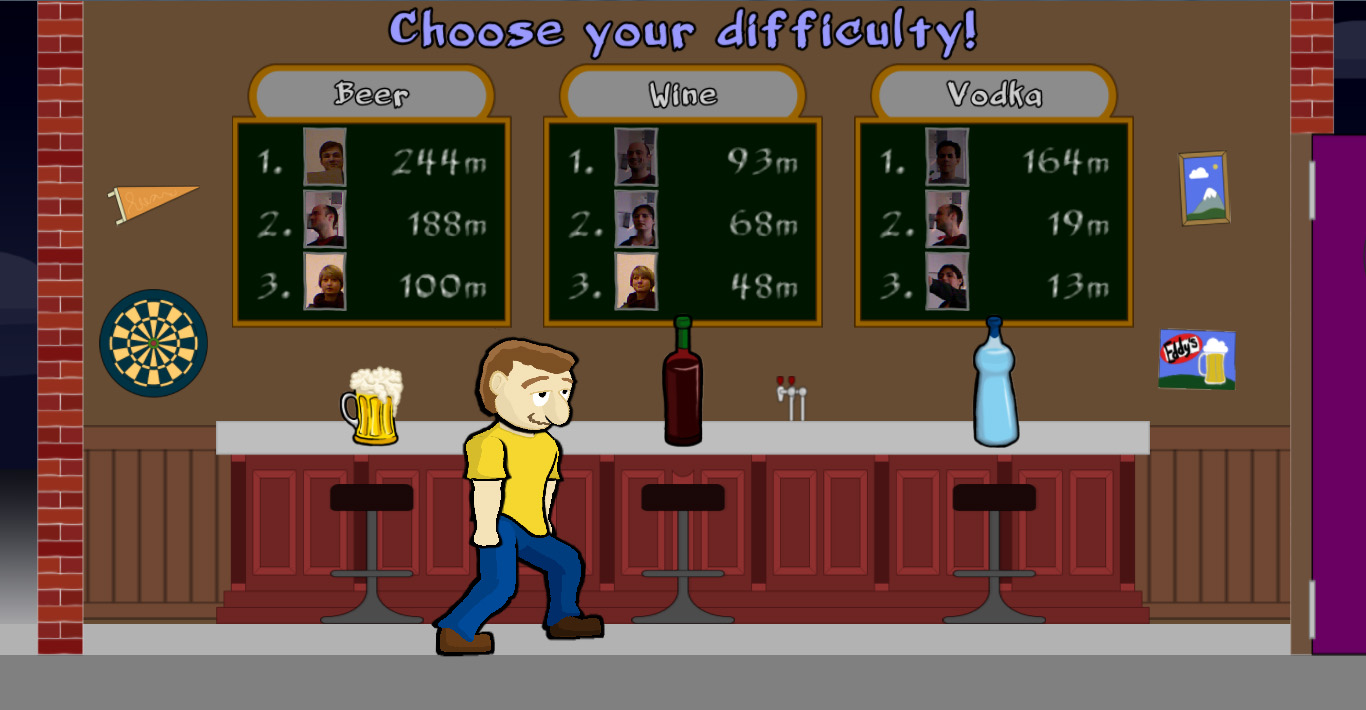
\includegraphics[width=\linewidth]{pictures/screenshot2.jpg}
  \caption{Insert a caption below each figure.}
  \label{fig:screenshot4}
\end{figure}
}
\item The narrative elements must be reduced to a minimum. There are no cutscenes, long texts etc. to tell the game's background. The animations, the players actions and keywords like ''distance'' give the game a humorous context.
\end{itemize}

\drunkened\ targets a joy of failing, that is, letting \ed\ eventually tumble and fall asleep. \eds\ tumbling is not implemented as an animation, but physics based, i.e. depending on \eds\ locomotion and angular velocity. This means, that failing varies from player to player, since they can take \ed\ into individual, often awkward, sleeping postures. This also attempts to compensate the fact, that \drunkened\ is a single player game, because spectators can have fun seeing others fail.

% =============================================================================
\section{Design Process}
% =============================================================================
\subsection{Project Outline}
After brainstorming we specified the project outline defining the setting of the installation, theme and main mechanics of the balance game and clarified the requirements. [picture of sketch]
Furthermore we created a fictional persona for whom we designed the game.
\subsection{Storyboarding and Interviews}
In order to explore possible scenarios for the deployment of our game we created story boards [picture of story board]. With these we approached three potential users and conducted semi-structured interviews to enquire about the need of such a form of entertainment in the given situation and also clarify the desirability of a  game such as \drunkened\ and the acceptability of its drinking context. From these interviews we learned that.. [TODO]
At a later point we invited participants to take part in an online vote, to make sure that this controversial subject was truly well accepted. Here we offered the option of a balance game featuring a dish washer balancing plates or a sleepwalking guy. A total of x people participated with a majority of votes for \drunkened.
\subsection{Paper Prototype and User Study}
Prior to implementation we performed user studies with a detailed paper prototype. Here we researched the comprehensibility of our menu, the users readiness to learn the controls and the need for hints and explanations. At this stage we made valuable observations on which we based our design decisions, such as to implement a menu which is operable with the same 
\subsection{Heuristic Prototype Evaluation}
After developing a first interactive prototype, we  analyzed our game regarding Nielsen’s 10 Usability Heuristics \cite{nielsen1995usability} and added two further principles, which we deemed essential for a casual game in public context.
%Here we wish to explain our additional principles.
%
%\begin{enumerate}
	%\item Motivation: All difficulty levels are available to play, so an advanced player does not need to stagger through all the easier stages first to reach a sufficiently challenging level. The highscores displayed above the level selection should provide the necessary motive to start another game and improve your score.
	%\item Learning curve (Additional Principle): A player can improve his performance and score, if he plays more often.
%\end{enumerate}
%Changes were made according to the results of this evaluation, as to the visibility of system status by adding a countdown at level start and including a highscore list for motivation.
A think aloud study was performed thereafter with several users of varying expertise, which lead to further improvements of the game according to Nielsen's heuristics. Among others we discovered the necessity of additional hints with both animated text and icons to ensure the user is constantly aware of his options and implemented a warning to be desplayed when the user leaves the optimal tracking region for error prevention. [picture of users]
\subsection{Implementation}
The game was implemented using OpenGL for the graphics and SimpleOpenNI to process input through the Kinect sensor.
% =============================================================================
\section{Conclusion}
% =============================================================================
The game is still under development. Right now, placeholder graphics are replaced and new obstacle elements are added to enhance the gameplay.

% =============================================================================
\section{Acknowledgements}
% =============================================================================
Special thanks go to our project supervisors J\"org M\"uller and Robert Walter for their help during development. Furthermore we wish to thank all volunteers who participated in interviews, experiments and play testing.
%%--------------------REMOVE FOLLOWING SECTIONS---------------------------------
%% =============================================================================
%\section{Copyright}
%% =============================================================================
%For publications in the CHI Extended Abstracts, copyright remains with the author.  
%The publication is not considered an archival publication; however, it does go into the ACM Digital Library. 
%Because you retain copyright, as the author you are free to use this material as you like, including submitting a paper based on this work to other conferences or journals.  
%Authors grant unrestricted permission for ACM to publish the accepted submission in the CHI Extended Abstracts without additional consideration or remuneration.
%
%% =============================================================================
%\section{Text formatting}
%% =============================================================================
%Please use an 8.5-point Verdana font, or other sans serifs font as close as possible in appearance to Verdana in which these guidelines have been set. 
%Arial 9-point font is a reasonable substitute for Verdana as it has a similar x-height. 
%Please use serif or non-proportional fonts only for special purposes, such as distinguishing source code text.
%Additionally, here is an example of footnoted text.\footnote{Use footnotes sparingly, if at all.}
%As stated in the footnote, footnotes should rarely be used.
%
%\subsection{Language, style, and content}
%% -----------------------------------------------------------------------------
%The written and spoken language of SIGCHI is English. 
%Spelling and punctuation may use any dialect of English (e.g., British, Canadian, US, etc.) provided this is done consistently. 
%Hyphenation is optional. 
%To ensure suitability for an international audience, please pay attention to the following:
%
%\begin{itemize}\compresslist
%\item 	
%Write in a straightforward style. 
%Use simple sentence structure. 
%Try to avoid long sentences and complex sentence structures. 
%Use semicolons carefully.
%\item 	
%Use common and basic vocabulary (e.g., use the word ``unusual" rather than the word ``arcane").
%\item 	
%Briefly define or explain all technical terms. 
%The terminology common to your practice/discipline may be different in other design practices/disciplines.
%\item 	
%Spell out all acronyms the first time they are used in your text. 
%For example, ``World Wide Web (WWW)".
%\item 	
%Explain local references (e.g., not everyone knows all city names in a particular country).
%\item 	
%Explain ``insider" comments. 
%Ensure that your whole audience understands any reference whose meaning you do not describe (e.g., do not assume that everyone has used a Macintosh or a particular application).
%\item 	
%Explain colloquial language and puns. 
%Understanding phrases like ``red herring" requires a cultural knowledge of English. 
%Humor and irony are difficult to translate.
%\item 	
%Use unambiguous forms for culturally localized concepts, such as times, dates, currencies and numbers (e.g., ``1-5-97" or ``5/1/97" may mean 5 January or 1 May, and ``seven o'clock" may mean 7:00 am or 19:00).
%\item 	
%Be careful with the use of gender-specific pronouns (he, she) and other gender-specific words (chairman, manpower, man-months). 
%Use inclusive language (e.g., she or he, they, chair, staff, staff-hours, person-years) that is gender-neutral. 
%If necessary, you may be able to use ``he" and ``she" in alternating sentences, so that the two genders occur equally often~\cite{Schwartz95}. 
%\end{itemize}
%
%
%% =============================================================================
%\section{Figures}
%% =============================================================================
%The examples on this and following pages should help you get a feel for how screen-shots and other figures should be placed in the template. 
%Be sure to make images large enough so the important details are legible and clear.
%
%\begin{figure}
  %\centering
  %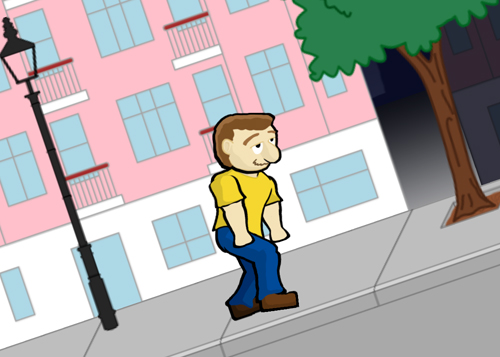
\includegraphics[width=\linewidth]{DrunkenEd.jpg}
  %\caption{Insert a caption below each figure.}
  %\label{fig:DrunkenEd}
%\end{figure}
%
%Your document may use color figures, which are included in the page limit; the figures must be usable when printed in black and white.
%You can use the \LaTeX's \texttt{marginpar} command to insert figures in the (right) margin side of the document (see \autoref{fig:marginparsample}).
%
%
%% =============================================================================
%\section{References and Citations}
%% =============================================================================
%Use a numbered list of references at the end of the article, ordered alphabetically by first author, and referenced by numbers in brackets \cite{Anderson92,Klemmer02,Mather00,Zellweger01}
%For papers from conference proceedings, include the title of the paper and an abbreviated name of the conference (e.g., for Interact 2003 proceedings, use Proc. Interact 2003). 
%Do not include the location of the conference or the exact date; do include the page numbers if available. 
%See the examples of citations at the end of this document. 
%
%Your references should be published materials accessible to the public.  
%Internal technical reports may be cited only if they are easily accessible (i.e., you provide the address for obtaining the report within your citation) and may be obtained by any reader for a nominal fee.  
%Proprietary information may not be cited. 
%Private communications should be acknowledged in the main text, not referenced  (e.g., [Robertson, personal communication]).
%
%% =============================================================================
%\section{Accessibility}
%% =============================================================================
%The Executive Council of SIGCHI has committed to making SIGCHI conferences more inclusive for researchers, practitioners, and educators with disabilities. As a part of this goal, the all authors are asked to work on improving the accessibility of their submissions. Specifically, we encourage authors to carry out the following five steps:
%\begin{enumerate}
	%\item Add alternative text to all figures
	%\item Mark table headings
	%\item Add tags to the PDF
	%\item Verify the default language
	%\item Set the tab order to ``Use Document Structure''
%\end{enumerate}
%Unfortunately good tools do not yet exist to create tagged PDF files from Latex. LaTeX users will need to carry out all of the above steps in the PDF directly using Adobe Acrobat, after the PDF has been generated.
 %
%For more information and links to instructions and resources, please see:
%{\url{http://chi2014.acm.org/authors/guide-to-an-accessible-submission}}.
%
%% =============================================================================
%\section{Producing and testing PDF files}
%% =============================================================================
%We recommend that you produce a PDF version of your submission well before the final deadline. 
%Besides making sure that you are able to produce a PDF, you will need to check that (a) the length of the file remains within the submission category's page limit, (b) the PDF file size is 4 megabytes or less, and (c) the file can be read and printed using Adobe Acrobat Reader. 
%Test your PDF file by viewing or printing it with the same software we will use when we receive it, Adobe Acrobat Reader Version 7. 
%This is widely available at no cost from~\cite{Acrobat7}.  
%Note that most reviewers will use a North American/European version of Acrobat reader, which cannot handle documents containing non-North American or non-European fonts (e.g. Asian fonts).  
%Please therefore do not use Asian fonts, and verify this by testing with a North American/European Acrobat reader (obtainable as above). Something as minor as including a space or punctuation character in a two-byte font can render a file unreadable.
%
%
%% =============================================================================
%\section{Dummy text}
%% =============================================================================
%Lorem ipsum dolor sit amet, consectetur adipiscing elit. Duis ut eros semper lectus vehicula elementum. Vestibulum ante ipsum primis in faucibus orci luctus et ultrices posuere cubilia Curae; Aliquam quis mi sapien. Suspendisse potenti. Mauris ultrices euismod velit sed dictum. Nullam auctor, nulla tincidunt dapibus suscipit, velit leo convallis metus, vel commodo libero erat in dolor. In laoreet porttitor ligula, porta blandit lectus consequat quis. 
%
%Nam ut eros dui. Mauris volutpat elit metus, euismod pellentesque purus. In hac habitasse platea dictumst. Nullam consectetur lacinia interdum. Sed nec blandit nisi. Proin in nulla purus, sit amet iaculis tortor. Ut dapibus pellentesque nulla in interdum. Nunc at velit felis. Curabitur euismod neque eu orci varius in pharetra sem interdum. Morbi in mauris ac risus iaculis dapibus id in magna. Class aptent taciti sociosqu ad litora torquent per conubia nostra, per inceptos himenaeos.
%
%\marginpar{
%\begin{figure}
  %\begin{center}
  %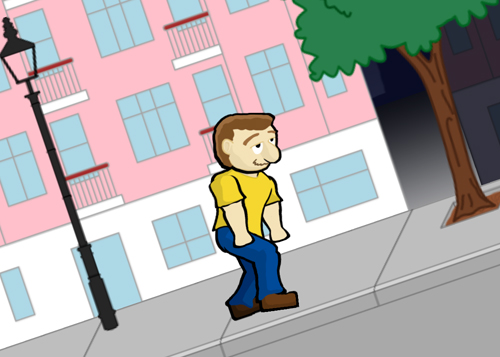
\includegraphics[width=\marginparwidth]{DrunkenEd.jpg}
  %\caption{A marginal figure.}
  %\label{fig:marginparsample}
  %\end{center}  
%\end{figure}
%}
%Aliquam consectetur quam sed odio varius vitae rhoncus urna fermentum. Phasellus viverra diam non justo porttitor varius. Integer ultrices accumsan lectus eget mollis. Nulla et leo sit amet nunc ornare rutrum sit amet ac dui. Cras vehicula accumsan purus nec fermentum. Mauris viverra condimentum metus, ut posuere quam laoreet nec. Phasellus massa tellus, ullamcorper nec porta sed, aliquet vitae nulla. Phasellus non tortor mauris. Cras ullamcorper egestas erat, vel rutrum elit viverra a. Donec in nisl ut est facilisis blandit. Quisque congue accumsan risus, ut venenatis magna vulputate vel. Nam commodo sapien vel mauris adipiscing nec dictum quam congue. Phasellus tempor vestibulum nisl quis blandit. Nullam condimentum auctor nibh, quis elementum libero tristique.
%
%
%
%\section{Acknowledgements}
%We thank all DUX 2003 publications support and staff who wrote this document originally and allowed us to modify it for this conference.
%This template was based on Manas Tungare's \texttt{chi.cls}, and rewritten by Luis A. Leiva.
%
%\section{References format}
%References must be the same font size as other body text.
%% REFERENCES FORMAT
%% References must be the same font size as other body text.

\balance
\bibliographystyle{acm-sigchi}
\bibliography{DrunkenEd}

\end{document}